\documentclass[a4paper,twoside]{article}

\usepackage{epsfig}
\usepackage{subfigure}
\usepackage{calc}
\usepackage{amssymb}
\usepackage{amstext}
\usepackage{amsmath}
\usepackage{amsthm}
\usepackage{multicol}
\usepackage{pslatex}
\usepackage{apalike}
\usepackage{SciTePress}
\usepackage[small]{caption}
\usepackage{epstopdf}
\usepackage[utf8]{inputenc}
\usepackage[ngerman]{babel}
\usepackage{url}
\usepackage{hyperref}
\usepackage{listings}


\lstdefinestyle{myCustomUseStyle}{
  stepnumber=1,
  numbersep=10pt,
  basicstyle=\footnotesize\ttfamily,
  tabsize=3,
  showspaces=false,
  showstringspaces=false,
  breaklines=true
}

\subfigtopskip=0pt
\subfigcapskip=0pt
\subfigbottomskip=0pt

\pagestyle{plain}

\begin{document}

\title{\uppercase{Modellgetriebene Entwicklung einer mobilen Applikation mit JUSE4Android}}

\author{\authorname{Jano Espenhahn, Tobias Franz and Franziska Krebs}
\affiliation{Fachhochschule Brandenburg, Fachbereich Informatik und Medien}
\email{\{espenhah, franzt, krebsf\}@fh-brandenburg.de}
}

\keywords{MDA, UML, USE, OCL, Android}

\abstract{ein deutsches Abstract: Entwicklung einer Applikation, USE-Spezifikation zur Definition eines Klassendiagramms; OCL-Constraints oben drauf;Im Anschluss Generierung der Anwendung mit Hilfe von JUSE4Android. Untersuchung der Anwendung anhand bestimmter Fragestellungen   }{ein englisches Abstract}


\onecolumn \maketitle \normalsize \vfill
\pagestyle{plain}
\section{\uppercase{Einleitung}}
\label{sec:introduction}
\noindent Zitat Test
\cite{SilvaMasterThesis}

\section{\uppercase{Beschreibung der Anwendung}}
\noindent
Das Beispiel wurde aus dem Artikel \cite{Gui06} entnommen. Es handelt sich um ein fiktives Programm der Regierung zur Kontrolle der Eispartikel in der Luft. Wenn die Konzentration zu niedrig ist, bedeutet das, dass die Bevölkerung zu wenig Eiscreme isst, was eine Menge an Risiken für die Umwelt und die öffentliche Ordnung darstellt. Um die Eispartikel in der Luft zu überwachen, hat der Staat Kontrollstationen im gesamten Land verteilt aufgestellt. Für jede Station gibt es einen festgelegten Zielwert der Eispartikel. Der aktuelle Wert weicht in der Regel vom Zielwert ab. 
\\
Die Anwendung ermöglicht es neue Stationen mit Zielwerten aufzunehmen und alte Stationen zu löschen. Außerdem gibt es die Möglichkeit eine Adresse zu einer Station anzugeben. Eine Adresse ist im Nachhinein auch wieder entfernbar. Die Erfassung von beliebig vielen Einträgen zu einer Station ist ebenfalls möglich. Auch Einträge lassen sich im Nachhinein wieder entfernen. Zudem wird für jeden Eintrag, nach Eingabe des aktuellen Wertes die Abweichung zum Zielwert angezeigt.


\section{\uppercase{Vorstellung USE}}
\noindent
UML based Specifiation Environment (USE) wird zur Spezifikation von Informationssystemen verwendet und wurde an der Universität Bremen entwickelt. Neben dem Einsatz für Fallstudien, wird USE vor allem in der Lehre an Hochschule wie z. B. MIT, Cambridge, University of Edinburgh und University of Lisbon eingesetzt.  USE basiert auf einer Teilmenge der Unified Modeling Language (UML) und der Object Constraint Language (OCL). Eine USE-Spezifikation besteht aus einer textuellen Beschreibung eines Modells, bei der Eigenschaften aus UML-Diagramm verwendet werden. Weitere Integritätsausdrücke für ein Modell können durch die OCL definiert werden. \cite{Use07}
%Die OCL wird im späteren Kapitel (TODO) vorgestellt. 
\\

Die Abbildung~\ref{fig:Grafik1} veranschaulicht den Workflow für eine USE-Spezifikation. Ein Entwickler spezifiziert ein plattformunabhängiges USE-Modell, welches ein System beschreibt und nutzt dafür UML- und OCL-Ausdrücke. Mithilfe von USE ist es ihm möglich, die bestimmten Anforderungen an sein System auf Erfüllung mit dem Modell zu validieren.

\begin{figure}[!h]
	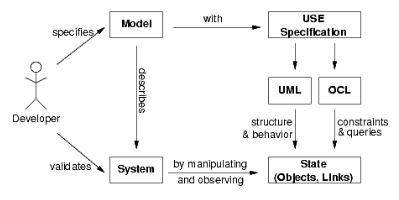
\includegraphics[scale=.7]{pics/USE_workflow.jpg}
	\caption{Workflow einer USE-Spezifikation \cite{Data07}}
	\label{fig:Grafik1}
\end{figure}

\subsection{Spezifikation} 
\label{ssec:specification}

Die textuelle Beschreibung eines Modells mit USE beginnt immer mit der Definition eines Modell-Namens. In diesem Fall ist das \textit{IceCream}. Im Anschluss folgen Klassendefinitionen mit ihren jeweiligen Attributen und Methoden. Im Beispiel hat die Klasse \textit{Station} das Attribut \textit{name} und die Operation \textit{entries} ohne Übergabeparameter. Die nachfolgenden Code-Ausschnitte verwenden lediglich UML.

\lstset{basicstyle=\tiny,style=myCustomUseStyle}
\begin{lstlisting}
model IceCream

class Station
	attributes
		name			: String
		target		: Integer
	operations
		entries()	: Set(Entry) = self.records->asSet
end
\end{lstlisting}

Klassen können untereinander in Abhängigkeit stehen. Für diese Abhängigkeiten sind Assoziationen vorgesehen. Um eine Assoziation auszudrücken, wird zuerst eine weitere Klasse \textit{Address} eingeführt.

\begin{lstlisting}
class Address
	attributes
		street	: String
		postCode	: Integer
end
\end{lstlisting}

Für das dem Artikel zugrunde liegende Beispiel kann eine Station entweder eine oder keine Adresse haben.

\begin{lstlisting}
association Station_Address between
	Station[ 1 ] 
	Address[ 0..1 ] role place
end
\end{lstlisting}

\textit{Station\_Address} ist dabei der Name der Assoziation und das Attribut \textit{place} nimmt in der Klasse \textit{Station} die Rolle für die Adresse ein. Zum gesamten USE-Modell gehören weiterhin noch die Klasse \textit{Entry} und die Assoziation \textit{Station\_Entry}.

\begin{lstlisting}
class Entry
	attributes
		date		: CalendarDate
		actual	: Integer
		variance	: Integer
	operations
		variance(): Integer = actual - station.target	
end

association Station_Entry between
	Station[ 1 ] role station
	Entry[ * ] role records
end
\end{lstlisting}

Zur Vervollständigung des Modells gehört außerdem eine aus der Arbeit \cite{SilvaMasterThesis} entnommene Klasse \textit{CalendarDate}.

\subsection{Erweiterung durch OCL} 
\label{ssec:ocl}
Als Bestandteil der UML ist die OCL ebenfalls als Spezifikation zur Modellierung von Softwareartefakten zu verstehen. Die Entwicklung der OCL wurde angetrieben durch den Wunsch, zusätzliche Modelleigenschaften - welche nicht mithilfe grafischer Elemente ausgedrückt werden können - festlegen zu können. \cite[S.5ff]{OCLFormal} Da diese Aspekte eindeutig und für alle Akteure verständlich sein sollen, wurde die OCL als eine formale und dennoch gut lesbare Sprache konzipiert. Das Vokabular der aktuell in Version 2.4. bereitgestellten Spezifikation ist sehr umfänglich und wird u.a. für die folgenden Zwecke genutzt: \begin{itemize}
\item als Abfragesprache
\item zur Definition von Invarianten
\item zur Beschreibung von Vor- und Nachbedingungen von Operationen 
\item zur Definition von Ableitungsregeln für Attribute
\item zur Definition von Restriktionen für Operationen
\end{itemize} 
Im Folgenden werden die OCL-Konstrukte erläutert, welche zur textuellen Beschreibung von Bedingungen im IceCream Beispiel verwendet wurden.  HINWEIS: keine context Schlüsselwort, da die Aussagen innerhalb der Klassen spezifiziert werden. Annotationen sind JUSE4Android spezifisch und nicht Bestandteil der OCL
Für die Klassen Station und Entry wurden die Invarianten \textit{TargetValueCannotBeNegative} und \textit{ActualValueCannotBeNegative} definiert. Diese repräsentieren Aussagen, welche für die Instanzen der jeweiligen Klasse zu jeder Zeit wahr sein müssen. \cite[S.188]{OCLFormal}
\begin{lstlisting}
@TargetValueCannotBeNegative(rationale="The defined target value of a station cannot be smaller than 0")
		inv TargetValueCannotBeNegative:
			target>=0
			
@ActualValueCannotBeNegative(rationale="The actual value measured at a station cannot be smaller than 0")
		inv ActualValueCannotBeNegative:
			actual>=0
\end{lstlisting}

Die Annotation bietet die Möglichkeit, die Invariante zu bezeichnen und näher zu erläutern. Nach dem Schlüsselwort \textit{inv} folgt erneut der Bezeichner. 
\subsection{USE-Tool}

Um eine Spezifikation auf nicht-formale Anforderungen zu validieren, kann ein Modell mithilfe des USE-Tools animiert werden. Direkt nach dem Import eines Modells erhält man vom Tool ein Feedback über die Validität der UML- und OCL-Definitionen. Neben der Validierung bietet das Tool weitere Möglichkeiten, wie z. B. die Visualisierung eines Klassen-, Sequenz- oder Objektdiagramms. In der Abbildung~\ref{fig:Grafik2} finden sich die im Kapitel~\ref{ssec:specification} definierten Klassen und Assoziationen als Klassendiagramm wieder.

\begin{figure}[!h]
	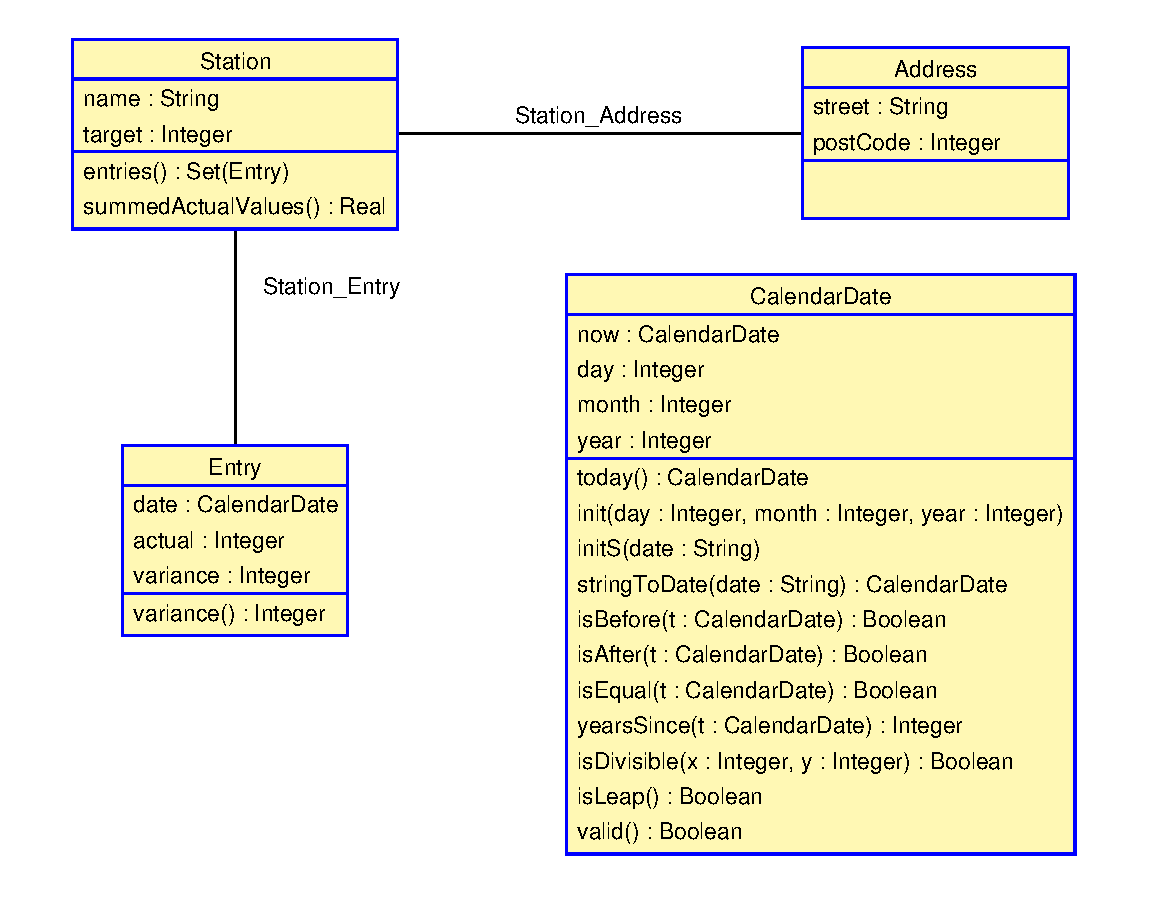
\includegraphics[scale=.4]{pics/USE_class_diagramm.pdf}
	\caption{Klassendiagramm für das Beispiel}
	\label{fig:Grafik2}
\end{figure}


\section{\uppercase{JUSE4Android}}
Dieser Abschnitt 

\subsection{Vorstellung}
Entstanden in Masterarbeit von ... 
db4o ist scheiße
Api-Level 17


\subsection{Untersuchung der erstellten Applikation}
Das Tool JUSE4Android erstellt aus dem Use-File eine Android-Applikation, welche sich durch folgende Schichten definiert: \textbf{Persistenz-Schicht, Presentations-Schicht, Model-Schicht(Business Logik)}. Dabei wurde konsequent das Model-View-View-Model Entwurfsmuster verwendet. Somit ist das Austauschen der Oberfläche theoretisch möglich.\\
Das vorherrschende Architekturmuster ist das Naked-Object-Pattern. Dieses definiert 3 Prinzipien. 1.) Die gesamte Geschäftslogik wird in Domänen Objekten gekapselt, 2.) Die Benutzeroberfläche ist eine direkte Repräsentation dieser Objekte und 3.) die Benutzeroberfläche kann oder wird direkt aus der Definition dieser Objekte erstellt. Diese 3 Prinzipien, werden von JUSE4Android vollständig umgesetzt. Zudem werden die Domänen Objekte direkt in eine Objekt Orientierte Datenbank gespeichert.\\
Der Programmfluss wird über die 4 grundlegenden Datenbankoperationen \textbf{C}reate \textbf{R}ead \textbf{U}pdate \textbf{D}elete gesteuert. Dabei werden neue Objekte sowohl in der Datenbank als auch der View verändert oder neu erstellt.\\
Master-Detail

\subsection{Generierter Code und zusätzliche Funktionalität}
Der aus der USE-Definition generierte Code ist in einer Paketstruktur gegliedert und hält die gängigen Code-Konventionen ein. Negativ muss erwähnt werden, dass dieser nur geringfügig kommentiert wurde und teilweise verschiedene Sprachen für die Kommentare verwendet wurden. Alles in allem ist der Code für einen Fortgeschrittenen Java/Android Entwickler nachvollziehbar und verständlich. Negativ ist zu betrachten, dass nur nach der Generierung manuelle Anpassungen oder zusätzliche Funktionalitäten vorgenommen werden können. Diese werden dementsprechend bei einer erneuten Generierung wieder überschrieben. Ebenfalls ist keine Möglichkeit vorgesehen, geschützte Bereiche zu definieren. Auch das Auslagern von manuellem Code in separate Dateien kann nicht vorgenommen werden, da der gesamte Code, mit Ausnahme von wenigen vordefinierten Standardklassen dynamisch durch die Applikation generiert wird. Somit ist eine Trennung von generiertem Code und manuellem Code nicht möglich. 

To Do: Bremen Tool sagt, das Modell sei valide; JUSE4Anroid: keine Generierung aufgrund der Definition von abgeleiteten Attributen

\subsection{Veränderungen der Benutzeroberfläche}
Durch die Verwendung des MVVM Musters ist die Veränderung oder der Austausch der Benutzeroberfläche theoretisch möglich. Dabei ist aber zu unterscheiden zwischen dem Austausch der gesamten oder einem Teil der Oberfläche und dem Anpassen und Verändern des Designs.\\
Die Anpassung des Designs ist schon durch die Gestaltungsmechanismen des Betriebssystems Android ohne Probleme möglich. Ebenfalls können verwendete Grafiken einfach ausgetauscht werden. Dies ist sogar vor der Generierung möglich.\\
i.	Einfügen einer alternativen View für die Varianz-Abweichung


Annotationen 

\section{Zusammenfassung und Fazit}
JUSE4Anroid zu starr; möglicherweise geht es in die Richtung der Generierung von Softwarekomponenten, im Gegensatz zur Generierung einer vollständigen Applikation
\vfill
\bibliographystyle{apalike}
{\small
\bibliography{bib/literature}}

\section*{\uppercase{Anhang}}

\noindent 
USE-Spezifikation, welche zur Generierung genutzt wird

\textit{$\backslash$section*\{APPENDIX\}}


\vfill
\end{document}

